\chapter{Elección de un software wiki}
\label{chapter:eleccion-software-wiki}

\begin{center}
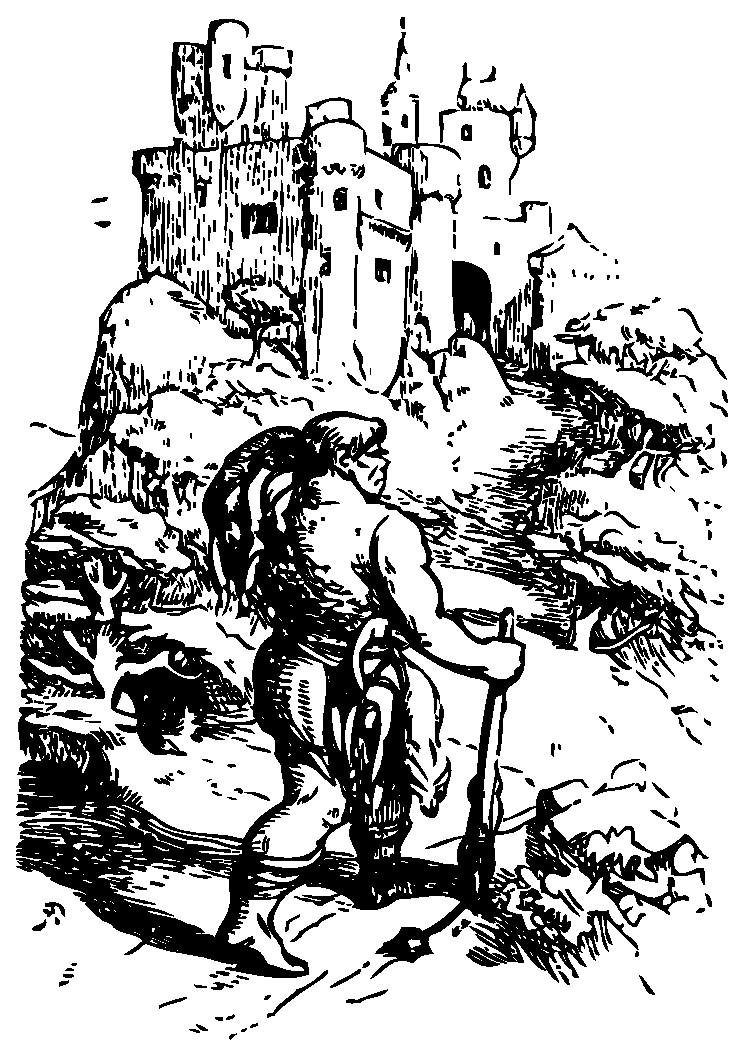
\includegraphics[scale=0.4]{../graphics/johnny_automatic_giant_going_to_castle.eps}
\end{center}

\lettrine{E}{n este capítulo} se analizarán las necesidades que tiene el proyecto \alma{} y se explicarán las causas del porqué de la elección de \tiki{} como herramienta principal frente a otras alternativas similares. Para finalizar se dará una visión genérica a las características más importantes de dicho \textit{software} y se informará al lector de los enlaces de interés para expandir su conocimiento sobre la plataforma.

\section{¿Qué necesidades tiene ALMA?}

A lo largo de todo el capítulo anterior se han ido razonando las motivaciones que tiene \alma{} siguiendo el modelo de las comunidades de práctica. Intuitivamente sabemos que la índole de este proyecto queda englobada en un entorno educativo que involucra grupos de usuarios trabajando alrededor de una temática concreta. Por lo tanto, es lógico pensar qué tipo de herramienta vamos a utilizar para implementar el concepto y para ello nos debemos preguntar por las necesidades concretas que debe responder el \textit{software}. A continuación, se listan los requisitos más importantes que consideramos a tener en cuenta:

\begin{itemize}
\item \textit{Wikis}: Dado que este es el pilar fundamental en el que se basan las comunidades de práctica, necesitamos que el \textit{software} que elijamos posea una implementación robusta de la filosofía \textit{wiki}. 

\item \textit{Gestión excelente de grupos y permisos asociados a ellos}: Una implementación correcta en la gestión de los grupos y sus permisos nos permite dividir las comunidades de práctica en distintos ámbitos (quizá no interese que los alumnos que pertenecen a una asignatura de \q{Circuitos Eléctricos} se mezclen con los alumnos que pertenecen a la asignatura de \q{Estadística}, ni que tampoco puedan modificar los elementos sobre los que estén trabajando estos últimos).

\item \textit{Facilidad en la instalación, mantenimiento y manejo}: Buscamos que nuestro \textit{software} no posea ninguna complejidad a la hora de instalarlo, que use componentes robustos y que, en general, el manejo sea sencillo (que no tiene porqué significar necesariamente que sea simple).

\item \textit{Automatización}: Es probable que si la plataforma es usada por mucha gente dicha gestión, por parte de un administrador, deje de ser algo trivial (asignación de permisos, creación de nuevas comunidades de práctica, establecer usuarios a diferentes grupos\ldots).

\item \textit{Robustez}: ¿Podemos estar seguros de que la plataforma soportará una gran cantidad de usuarios?

\item \textit{Que sea adaptable}: El \textit{software} debe permitir crear cualquier estructura posible. En nuestro caso el concepto de las comunidades de práctica como se mostró en la \figureref{comunidades_de_practica} en el \chapterref{estado-cuestion}.
\end{itemize}

\section{¿Qué herramientas existen?}

En el mercado actualmente podemos encontrar muchas propuestas que nos permiten implementar de múltiples maneras y formas un sistema de aprendizaje virtual (\textit{e-learning}). La denominación que reciben este tipo de \textit{software} es: \lms{}. Y es un \textit{software} que se instala en un servidor web y que se emplea para administrar, distribuir y controlar las actividades de formación no presencial de una institución o organización \cite{web:lms}.

Las principales funciones del \lms{} son: gestionar usuarios, recursos, así como materiales y actividades de formación. También se encargan de administrar el acceso al mismo, controlar y hacer seguimiento de los procesos de aprendizaje, realizar evaluaciones, generar informes, gestionar servicios de comunicación como foros de discusión\ldots{} En cambio, generalmente, no incluyen posibilidades de autoría, es decir, que se pueda crear contenidos propios, sino que se centra en gestionar contenidos creados por fuentes diferentes.

\alma{}, \textit{per se}, no utiliza todas las características a las que se adscriben los \lms{}. Por ejemplo, el hecho de que no suelen incluir contenidos generados por los propios usuarios es algo que contradice expresamente la naturaleza de este proyecto. Este pequeño detalle, como veremos más adelante, nos hizo descartar algunas propuestas por no cumplir con los requisitos necesarios.

Por lo tanto, si \alma{} no se puede categorizar dentro de un \lms{} propiamente dicho (aún compartiendo muchas de sus ideas), ¿qué es entonces? Podríamos responder que es un híbrido entre un \lms{} y un \cms{} \cite{web:cms}.

Un \cms{} es un programa que, al igual que un \lms{}, se puede instalar en un servidor web y permite, de manera sencilla, la creación y la administración de contenidos (principalmente para ser consumidos en páginas web) por parte de los administradores, editores, participantes y demás roles.

En \alma{} los contenidos son creados por los propios usuarios, otras veces, por alguien externo. Por lo tanto, ¿qué propuestas encontramos en el mercado que más o menos se ajusten a un híbrido de un \lms{} y un \cms{}? Se listan a continuación las opciones más relevantes:

\begin{itemize}
\item WebCT o BlackBoard
\item Moodle
\item MediaWiki
\item \tiki{}
\end{itemize}

WebCT, conocido también como BlackBoard \cite{web:blackboard}, es, por definición expresa, el sistema que ha determinado, tal y como lo conocemos, las bases de los \lms{} de manera concreta y del aprendizaje virtual (\textit{e-learning}) en general. Nuestra universidad lo usa en múltiples cursos y asignaturas de las diferentes carreras que se imparten \cite{web:webct-uah}.

No negamos que se trata de un \textit{software} que es bastante competente en su terreno, pero la mayor desventaja que tiene es que su licencia es privativa y por ello el usuario no tiene ningún derecho a poder copiar, estudiar, modificar y redistribuir el código de la plataforma \cite[pág~2]{paper:innovamos}. Es más, tendríamos que pagar una licencia por el uso de la misma. Por lo tanto desde el principio consideramos que no era una opción plausible. 

La alternativa más conocida a WebCT es Moodle \cite{web:moodle}. Posee muchas de las características del primero más algunas suyas propias. Nuestra universidad también lo usa en determinadas asignaturas \cite{web:moodle-uah}. Sin embargo, tampoco es una opción a tener en cuenta porque principalmente está centrado en distribuir cursos (o lecciones) provenientes de una fuente central (el profesor por ejemplo) y unos alumnos trabajando sobre esos materiales. Realmente se pueden ver como una ayuda a la clase, o como una forma de sustituirla, pero no para complementarla de manera creativa a como lo propone el concepto de las comunidades de práctica. Por lo que también quedó descartada.

MediaWiki \cite{web:mediawiki} es quizá la más conocida de las expuestas, puede que no de manera directa, pero es el \textit{software} que corre la Wikipedia \cite{web:wikipedia}.
Como su propio nombre indica se centra en las \textit{wikis} de manera exclusiva (lo cual es bastante positivo porque es uno de los requisitos que pedimos para \alma{}). Otro aspecto es que se puede instalar muy fácilmente en cualquier servidor que cumpla unos requisitos mínimos. Además posee una comunidad de usuarios bastante amplia y hay muchos manuales que explican como configurar y modificar el propio \textit{software}. Sin embargo, como características negativas es que la gestión y la administración de los usuarios no es tan trivial, tampoco se pueden crear grupos aislados de usuarios ni controlar los accesos a las diferentes páginas \textit{wikis} de una manera selectiva, y no hay posibilidad de automatizar ciertas tareas de gestión rutinarias. Por lo tanto es otra opción que descartamos.

\section{¿Por qué se escogió TikiWiki?}

\begin{figure}
\centering

\includegraphics[scale=0.75]{../graphics/tiki-logo.png}
\caption{Logotipo de Tikiwiki.}\label{fig:tikiwiki_logo}
\end{figure}

De las cuatro opciones que se han presentado, la última que queda es \tiki{}. Fue escogida por los siguientes motivos (responde a muchas de las peticiones que pusimos antes y añade más características que no habíamos pensado pero que, sin embargo, nos son útiles):

\begin{itemize}
\item \textit{Versátil}: El diseño de \tiki{} es lo que se conoce como un \q{todo-en-uno}, es decir, aglutina muchas características en un sólo \textit{software}. Esto es positivo porque actualmente \alma{} utiliza las \textit{wikis} como medio para crear las comunidades de práctica, pero, en algún futuro se podrían utilizar otras herramientas que sirviesen para el mismo propósito, por ejemplo, foros de discusión. Al tener \tiki{} integradas las \textit{wikis}, los foros, los \textit{blogs}, galerías de imágenes, mapas\ldots{} dentro del propio \textit{software}, nos olvidamos de tener que instalar complementos (\textit{plug-ins}) u otras herramientas externas para conseguir el mismo efecto.

\item \textit{Fiable}: Muchos proyectos de código abierto (y otros tantos comerciales) utilizan \tiki{} como motor principal para gestionar sus \textit{wikis} (y otras necesidades). Como ejemplo importante que utilice \tiki{} encontramos al motor de 3\textsc{d} Ogre \cite{web:ogre-tikiwiki, web:tikiwikis-destacadas}.

\item \textit{Flexible}: \tiki{} se puede adaptar a cualquier necesidad ya que, al incorporar una gran cantidad de opciones, puede ser utilizado como una \textit{wiki}, como un \textit{blog} para una persona, un gestor de errores en programación (\textit{bug tracker}),  una comunidad de usuarios, un portal de noticias, una web corporativa \cite{web:tiki-use-cases}\ldots{} La imaginación es nuestro límite.

\item \textit{Profiles}: Como apoyo al punto anterior, y debido a que \tiki{} posee más de 1500 opciones de configuración distintas, surgieron los \profiles{}. Éstos permiten modificar cualquier opción posible de la plataforma de \tiki{} de una manera sencilla y eficaz utilizando ficheros de \q{texto plano}. Esta fue la característica principal de la elección de \tiki{} como \textit{software} y con la que se consiguió implementar \alma{} con éxito.

\item \textit{Perspectivas}: Otra de las habilidades de este \textit{software} que destaca por si sola es que permite, por ejemplo, que para un mismo usuario la experiencia usando el \textit{software} de \tiki{} sea completamente diferente dependiendo de las acciones que realice.

\item \textit{Excelente gestión de usuarios y de permisos}: Con \tiki{} se obtiene una jerarquía de permisos muy fina y detallada, se pueden aplicar de manera global a todos los usuarios, o pueden ser concretos tanto a un usuario como a un grupo o bien a un recurso (una \textit{wiki}) permitiendo dar acceso o denegarlo acorde a las necesidades que se tengan.

\item \textit{Facilidad de instalación}: Para funcionar \tiki{} sólo necesita un servidor capaz de ejecutar código en \php{} 5 \cite{web:php} y una base de datos \textsc{m}y\textsc{sql} \cite{web:mysql} para guardar la información.

\end{itemize}

\subsection{Información de interés sobre TikiWiki}

A continuación dejamos al lector interesado en obtener más información una serie de enlaces importantes sobre \tiki{} y que varían desde la descarga de el propio \textit{software} hasta casos complejos de configuración, a saber:

\begin{itemize}
\item Información básica de la plataforma (\url{http://tiki.org}): Aquí podemos descargar el \textit{software} y obtener información básica de sus características principales. Es útil para averiguar si \tiki{} se ajusta a nuestras necesidades o no.

 \item Documentación genérica (\url{http://doc.tiki.org}): Esta página está orientada a la obtención de información por parte del administrador de la plataforma. Cualquier necesidad que surja a la hora de configurar el \textit{software}, aquí es probable que se encuentre la respuesta.
 
 \item Desarrollo (\url{http://dev.tiki.org}): Esta \textit{wiki} está preparada para los desarrolladores del código ya que se muestran las últimas novedades que se producen en el código fuente de \tiki{}, así como también nuevas características que se añadirán a versiones futuras, implementaciones que se han realizado y en general cualquier tipo de documentación útil para la gente que quiera programar.

 \item \profiles{} (\url{http://profiles.tiki.org}): Aquí se puede encontrar toda la información importante sobre la información relacionada con la configuración, desarrollo y creación de los \profiles{}. También es un punto de intercambio de nuevos \profiles{} que hayan creado otros usuarios. Instamos al lector interesado a que visite esta página web para obtener una información más detallada sobre esta herramienta.

 \item Canal de \textsc{irc} (\url{http://webchat.freenode.net/?channels=tikiwiki}): En este canal de \textsc{irc} se alojan los principales \q{sabios de \tiki{}} que nos pueden ayudar siempre que lo necesitemos.
\end{itemize}
